

\tikzset{every picture/.style={line width=0.75pt}} %set default line width to 0.75pt        

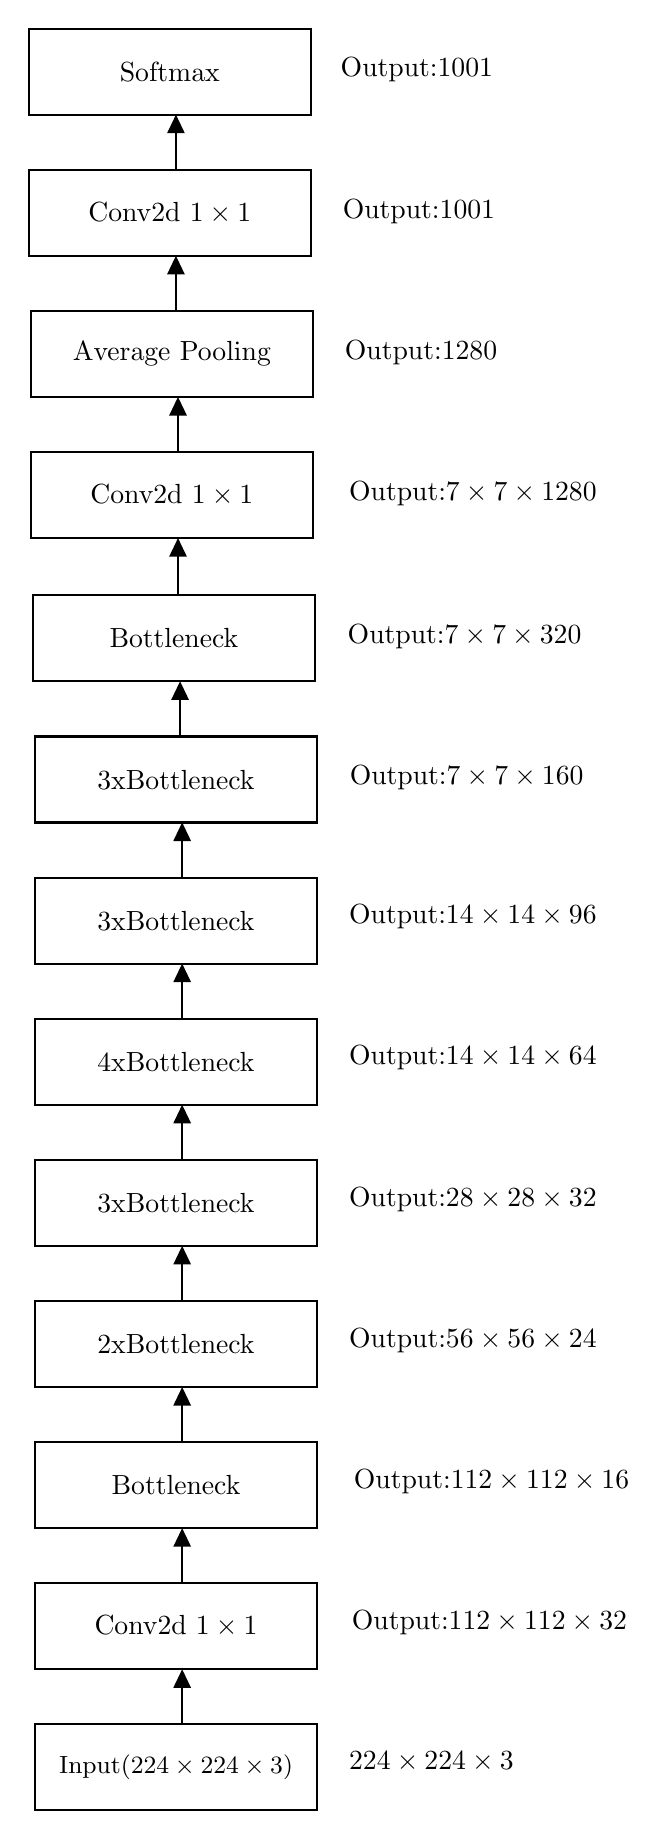
\begin{tikzpicture}[x=0.75pt,y=0.75pt,yscale=-1,xscale=1]
%uncomment if require: \path (0,948.6666870117188); %set diagram left start at 0, and has height of 948.6666870117188

%Flowchart: Process [id:dp9253173394290999] 
\draw   (98,897) -- (233.93,897) -- (233.93,938.43) -- (98,938.43) -- cycle ;
%Flowchart: Process [id:dp47578347996398307] 
\draw   (98,829) -- (233.93,829) -- (233.93,870.43) -- (98,870.43) -- cycle ;
%Straight Lines [id:da2925025767777827] 
\draw    (168.93,897.43) -- (168.93,872.43) ;
\draw [shift={(168.93,870.43)}, rotate = 450] [fill={rgb, 255:red, 0; green, 0; blue, 0 }  ][line width=0.75]  [draw opacity=0] (8.93,-4.29) -- (0,0) -- (8.93,4.29) -- cycle    ;

%Flowchart: Process [id:dp5382364848384393] 
\draw   (98,761) -- (233.93,761) -- (233.93,802.43) -- (98,802.43) -- cycle ;
%Straight Lines [id:da06940381159807729] 
\draw    (168.93,829.43) -- (168.93,804.43) ;
\draw [shift={(168.93,802.43)}, rotate = 450] [fill={rgb, 255:red, 0; green, 0; blue, 0 }  ][line width=0.75]  [draw opacity=0] (8.93,-4.29) -- (0,0) -- (8.93,4.29) -- cycle    ;

%Flowchart: Process [id:dp21301144435418706] 
\draw   (98,693) -- (233.93,693) -- (233.93,734.43) -- (98,734.43) -- cycle ;
%Straight Lines [id:da45627711718103714] 
\draw    (168.93,761.43) -- (168.93,736.43) ;
\draw [shift={(168.93,734.43)}, rotate = 450] [fill={rgb, 255:red, 0; green, 0; blue, 0 }  ][line width=0.75]  [draw opacity=0] (8.93,-4.29) -- (0,0) -- (8.93,4.29) -- cycle    ;

%Flowchart: Process [id:dp7231968775803179] 
\draw   (98,625) -- (233.93,625) -- (233.93,666.43) -- (98,666.43) -- cycle ;
%Straight Lines [id:da7165121439179447] 
\draw    (168.93,693.43) -- (168.93,668.43) ;
\draw [shift={(168.93,666.43)}, rotate = 450] [fill={rgb, 255:red, 0; green, 0; blue, 0 }  ][line width=0.75]  [draw opacity=0] (8.93,-4.29) -- (0,0) -- (8.93,4.29) -- cycle    ;

%Flowchart: Process [id:dp20620702942862734] 
\draw   (98,557) -- (233.93,557) -- (233.93,598.43) -- (98,598.43) -- cycle ;
%Straight Lines [id:da10564528480224444] 
\draw    (168.93,625.43) -- (168.93,600.43) ;
\draw [shift={(168.93,598.43)}, rotate = 450] [fill={rgb, 255:red, 0; green, 0; blue, 0 }  ][line width=0.75]  [draw opacity=0] (8.93,-4.29) -- (0,0) -- (8.93,4.29) -- cycle    ;

%Flowchart: Process [id:dp6409642010028676] 
\draw   (98,489) -- (233.93,489) -- (233.93,530.43) -- (98,530.43) -- cycle ;
%Straight Lines [id:da583110185704452] 
\draw    (168.93,557.43) -- (168.93,532.43) ;
\draw [shift={(168.93,530.43)}, rotate = 450] [fill={rgb, 255:red, 0; green, 0; blue, 0 }  ][line width=0.75]  [draw opacity=0] (8.93,-4.29) -- (0,0) -- (8.93,4.29) -- cycle    ;

%Flowchart: Process [id:dp747253235525678] 
\draw   (98,421) -- (233.93,421) -- (233.93,462.43) -- (98,462.43) -- cycle ;
%Straight Lines [id:da9482962038382927] 
\draw    (168.93,489.43) -- (168.93,464.43) ;
\draw [shift={(168.93,462.43)}, rotate = 450] [fill={rgb, 255:red, 0; green, 0; blue, 0 }  ][line width=0.75]  [draw opacity=0] (8.93,-4.29) -- (0,0) -- (8.93,4.29) -- cycle    ;

%Flowchart: Process [id:dp47103409298757426] 
\draw   (97,353) -- (232.93,353) -- (232.93,394.43) -- (97,394.43) -- cycle ;
%Straight Lines [id:da30249651940608824] 
\draw    (167.93,421.43) -- (167.93,396.43) ;
\draw [shift={(167.93,394.43)}, rotate = 450] [fill={rgb, 255:red, 0; green, 0; blue, 0 }  ][line width=0.75]  [draw opacity=0] (8.93,-4.29) -- (0,0) -- (8.93,4.29) -- cycle    ;

%Flowchart: Process [id:dp5661311837160838] 
\draw   (96,284) -- (231.93,284) -- (231.93,325.43) -- (96,325.43) -- cycle ;
%Straight Lines [id:da5142446239913938] 
\draw    (166.93,352.43) -- (166.93,327.43) ;
\draw [shift={(166.93,325.43)}, rotate = 450] [fill={rgb, 255:red, 0; green, 0; blue, 0 }  ][line width=0.75]  [draw opacity=0] (8.93,-4.29) -- (0,0) -- (8.93,4.29) -- cycle    ;

%Flowchart: Process [id:dp8648151912409288] 
\draw   (96,216) -- (231.93,216) -- (231.93,257.43) -- (96,257.43) -- cycle ;
%Straight Lines [id:da21788225541174455] 
\draw    (166.93,284.43) -- (166.93,259.43) ;
\draw [shift={(166.93,257.43)}, rotate = 450] [fill={rgb, 255:red, 0; green, 0; blue, 0 }  ][line width=0.75]  [draw opacity=0] (8.93,-4.29) -- (0,0) -- (8.93,4.29) -- cycle    ;

%Flowchart: Process [id:dp5915277931570215] 
\draw   (95,148) -- (230.93,148) -- (230.93,189.43) -- (95,189.43) -- cycle ;
%Straight Lines [id:da2169186042376452] 
\draw    (165.93,216.43) -- (165.93,191.43) ;
\draw [shift={(165.93,189.43)}, rotate = 450] [fill={rgb, 255:red, 0; green, 0; blue, 0 }  ][line width=0.75]  [draw opacity=0] (8.93,-4.29) -- (0,0) -- (8.93,4.29) -- cycle    ;

%Flowchart: Process [id:dp09241683513730559] 
\draw   (95,80) -- (230.93,80) -- (230.93,121.43) -- (95,121.43) -- cycle ;
%Straight Lines [id:da3985231842573671] 
\draw    (165.93,148.43) -- (165.93,123.43) ;
\draw [shift={(165.93,121.43)}, rotate = 450] [fill={rgb, 255:red, 0; green, 0; blue, 0 }  ][line width=0.75]  [draw opacity=0] (8.93,-4.29) -- (0,0) -- (8.93,4.29) -- cycle    ;


% Text Node
\draw (165.96,917.71) node  [align=left] {{\small Input($\displaystyle 224\times 224\times 3$)}};
% Text Node
\draw (165.96,849.71) node  [align=left] {Conv2d $\displaystyle 1\times 1$};
% Text Node
\draw (289,915) node  [align=left] {$\displaystyle 224\times 224\times 3$};
% Text Node
\draw (317,848) node  [align=left] {Output:$\displaystyle 112\times 112\times 32$};
% Text Node
\draw (165.96,781.71) node  [align=left] {Bottleneck};
% Text Node
\draw (318,780) node  [align=left] {Output:$\displaystyle 112\times 112\times 16$};
% Text Node
\draw (165.96,713.71) node  [align=left] {2xBottleneck};
% Text Node
\draw (309,712) node  [align=left] {Output:$\displaystyle 56\times 56\times 24$};
% Text Node
\draw (165.96,645.71) node  [align=left] {3xBottleneck};
% Text Node
\draw (309,644) node  [align=left] {Output:$\displaystyle 28\times 28\times 32$};
% Text Node
\draw (165.96,577.71) node  [align=left] {4xBottleneck};
% Text Node
\draw (309,576) node  [align=left] {Output:$\displaystyle 14\times 14\times 64$};
% Text Node
\draw (165.96,509.71) node  [align=left] {3xBottleneck};
% Text Node
\draw (309,508) node  [align=left] {Output:$\displaystyle 14\times 14\times 96$};
% Text Node
\draw (165.96,441.71) node  [align=left] {3xBottleneck};
% Text Node
\draw (306,441) node  [align=left] {Output:$\displaystyle 7\times 7\times 160$};
% Text Node
\draw (164.96,373.71) node  [align=left] {Bottleneck};
% Text Node
\draw (305,373) node  [align=left] {Output:$\displaystyle 7\times 7\times 320$};
% Text Node
\draw (163.96,304.71) node  [align=left] {Conv2d $\displaystyle 1\times 1$};
% Text Node
\draw (309,304) node  [align=left] {Output:$\displaystyle 7\times 7\times 1280$};
% Text Node
\draw (163.96,236.71) node  [align=left] {Average Pooling};
% Text Node
\draw (284,236) node  [align=left] {Output:$\displaystyle 1280$};
% Text Node
\draw (162.96,168.71) node  [align=left] {Conv2d $\displaystyle 1\times 1$};
% Text Node
\draw (283,168) node  [align=left] {Output:$\displaystyle 1001$};
% Text Node
\draw (162.96,100.71) node  [align=left] {Softmax};
% Text Node
\draw (282,100) node  [align=left] {Output:$\displaystyle 1001$};


\end{tikzpicture}